\documentclass[11pt]{article}

\usepackage[utf8]{inputenc}
\usepackage[T1]{fontenc}
\usepackage[margin=1in]{geometry}
\usepackage{amsmath}
\usepackage{booktabs}
\usepackage{graphicx}
\usepackage{caption}
\usepackage{hyperref}
\usepackage[round, authoryear]{natbib}

\hypersetup{
    colorlinks=true,
    linkcolor=blue!50!black,
    citecolor=blue!50!black,
    urlcolor=blue!50!black,
}

\title{Short-term residential load forecasting at the portfolio level\\
       for a Spanish energy cooperative}
\author{Carlo M.\\ Universitat de Barcelona\\ \texttt{cvilchce15@alumnes.ub.edu}}
\date{\today}

\begin{document}
\maketitle

\begin{abstract}
\noindent
We document a portfolio-level short-term load forecasting pipeline for a
Spanish energy cooperative covering 16,764 residential households. The
forecaster is a recursive single-step LightGBM with five quantiles, trained
with early stopping on a temporal hold-out followed by a refit on the full
365-day window using the iteration count selected by validation
(\emph{refit-on-full}). Split conformal post-hoc calibration brings
empirical coverage of the 50\% and 90\% prediction intervals within
2~percentage points of nominal across three horizon buckets. Walk-forward
validation over 105 weekly folds yields a median MAPE of 4.88\% at
$h \leq 24$ and a 29.6\% lift over the persistence baseline at the same
horizon. The model underperforms persistence at $h \geq 72$
(lift $-25\%$ to $-32\%$), a structural consequence of recursive error
compounding that we document explicitly. We also contribute a complementary
behavioral segmentation toolkit ($k = 3$, silhouette $< 0.20$) for tariff
design applications, kept architecturally independent from the forecasting
pipeline.
\end{abstract}

% =====================================================================
\section{Introduction}
% =====================================================================

Short-term load forecasting drives day-ahead procurement, intraday balancing
and demand-response targeting in retail energy supply. For a small or
mid-sized energy cooperative serving residential customers, forecasting at
the \emph{portfolio} level (the sum of all customers' hourly consumption)
is the operationally relevant target: bulk energy is procured against the
aggregate, and imbalance settlement is computed against it. Forecasting
\emph{per customer} is unnecessary for procurement and infeasible at scale
on residential meters; segmentation \emph{between} those two extremes is a
question of architecture.

The hierarchical-forecasting literature \citep{wickramasuriya2019,
hyndman2021} suggests that forecasting subgroups (e.g.\ behavioral clusters
of customers) and reconciling their forecasts to the portfolio aggregate
can improve accuracy when subgroup signals carry distinct information not
captured by the aggregate. The trade-off is increased complexity, more
models, and a reconciliation step (BottomUp, MinT-OLS, or related
trace-minimization estimators) whose benefits depend on whether subgroup
heterogeneity is forecastable and stable across the validation window.

This work documents a pipeline that explicitly evaluates the
hierarchical-vs-portfolio trade-off and converges on a portfolio-only
architecture, with the residual segmentation contribution kept as an
independent commercial-side artefact rather than a forecasting input. We
report walk-forward MAPE, post-hoc conformal calibration of prediction
intervals, and lift over a strong persistence baseline. We document the
horizons at which the model wins and at which it loses, the latter being a
structural consequence of recursive single-step inference rather than a
hyperparameter pathology.

The contribution is methodological rather than novel-architectural: an
honest, reproducible pipeline with explicit limitations that other small
operators with the same constraints (residential portfolio, hourly meters,
limited tooling budget) can adopt or critique. A complementary
\emph{Pipeline~2}, built on the same dataset but architecturally
independent, returns a three-archetype k-means segmentation usable for
tariff design and demand response targeting.

% =====================================================================
\section{Data}
% =====================================================================

We use the GoiEner smart-meter dataset \citep{quesada2024goiener},
a publicly released hourly consumption panel of 25,559 supply points in
the Basque Country and other Spanish regions, of which 16,764 are
residential (CNAE-2009 code starting with 98). The dataset spans
2014-11-01 through 2022-06-30 with hourly resolution.

After data-quality filtering (minimum one year of valid hours per
household, maximum 20\% imputed observations, non-zero daily variance),
10,531~households retain a usable pre-2020 daily profile. The remaining
6,233 are dropped: 6,219 lack any pre-2020 observations and 14 have
constant readings across the day. Households included after filtering are
aggregated to a hourly portfolio panel by summation, yielding 21,671
hourly observations between 2018-01-01 and 2020-06-21 used for champion
training, plus the 2020-06-22 to 2022-06-30 validation window over which
the walk-forward is computed.

Hourly weather covariates (temperature, relative humidity, precipitation,
wind speed) are pulled from the Open-Meteo historical archive at three
geographic points (Bilbao, Pamplona, Madrid) and weighted by their share of
the cooperative's customer base (72.5\%, 13.8\%, 13.7\% respectively) to
produce a single portfolio-weighted hourly series. Spanish national
holidays are obtained from the \texttt{holidays} package and matched to
calendar dates.

The validation window is intentionally chosen to start in mid-2020 (after
the COVID-19 lockdown shock that ended on 2020-06-21) and to span the
2021-06-01 mandatory tariff reform (the 2.0TD time-of-use roll-out), so
the walk-forward straddles a known regime change. We address this regime
shift in the conformal calibration step by interleaving calibration and
test folds rather than splitting them temporally; details follow.

A central caveat: weather features are \emph{realized} (observed
historical) rather than forecast. In production, forecast weather would
replace the realized series; this paper evaluates methodology rather than
deployed accuracy. The same caveat applies in any retrospective
forecasting study using historical weather and is documented prominently
because it materially affects external validity.

% =====================================================================
\section{Pipeline 1 --- Methodology}
% =====================================================================

\subsection{Architecture: portfolio-only}

We forecast the hourly portfolio aggregate
$y_t = \sum_{i \in \text{customers}} y_{i,t}$ directly. Per-segment
forecasting was implemented and evaluated under a previous version of this
pipeline; we found that (i) the recursive single-step architecture cannot
exploit segment heterogeneity at long horizons because the median forecast
is fed back as a lag input and over 168 steps the segment trajectories
drift toward the mean; and (ii) the validation pinball loss on extreme
quantiles ($q = 0.05, 0.95$) for small segments is dominated by tail noise
on a 30-day window, producing premature early stopping at iteration counts
that did not extrapolate to the prediction horizon. The hierarchical
reconciliation step (MinT-OLS, BottomUp) yielded marginal portfolio-MAPE
improvements at $h = 25$--$72$ but degraded at $h \leq 24$ and $h = 168$,
and was therefore dropped together with the per-segment models. Pipeline~1
in this paper is the post-reframe portfolio-only configuration.

\subsection{Champion training: early stopping with refit-on-full}

For each quantile $q \in \{0.05, 0.25, 0.50, 0.75, 0.95\}$ we train one
LightGBM \citep{ke2017lightgbm} booster with quantile loss and recursive
single-step target $y_{t+1} \mid \text{features}(t)$. The target window is
strictly past at every fold (Section~3.4); we report training in two
phases.

\textbf{Phase 1} runs early stopping on a temporal hold-out. The supervised
frame at each training cutoff is split chronologically into 335 days of
training and 30 trailing days of validation, with the validation
strictly after the training set. \texttt{lgb.train} runs with patience
$=$ 100 boosting rounds and a ceiling of 2,500 iterations; the call returns
the early-stopping best iteration $K$. Patience was raised from the LightGBM
default (50) after the previous version's walk-forward exhibited 8.9\% of
fits stopping under 100 iterations on quantile losses dominated by
validation-window noise; raising patience to 100 reduces the rate but does
not eliminate it (Section~5).

\textbf{Phase 2} retrains a fresh booster on the entire 365-day window
(training plus the 30-day validation hold-out) for exactly $K$ boosting
rounds, with no validation set and no callbacks. This recovers the 30 days
sacrificed to early stopping while preserving the iteration count selected
by honest validation. The phase-2 booster is the model artefact saved and
used downstream. The information that determined $K$ is discarded after
phase~1 by construction.

The split is strictly temporal at every step. We assert
$\text{valid}_{\min} > \text{train}_{\max}$ before training and abort if
the invariant is violated. We verified empirically that across all 105
walk-forward folds the phase-2 maximum timestamp is at least 2~hours
before the fold's issue time, so phase~2 cannot use any data posterior
to the cutoff.

LightGBM hyperparameters are: \texttt{learning\_rate $=$ 0.05},
\texttt{num\_leaves $=$ 63}, \texttt{min\_data\_in\_leaf $=$ 50},
\texttt{feature\_fraction $=$ 0.9}, \texttt{bagging\_fraction $=$ 0.9},
\texttt{bagging\_freq $=$ 5}, fixed across quantiles. Iteration counts of
the five champion models on the 2020-06-22 cutoff are
$\{784, 642, 510, 184, 305\}$ for $q = \{0.05, 0.25, 0.50, 0.75, 0.95\}$
respectively (\texttt{output/05\_lgb\_training\_summary.csv}). The
asymmetric distribution (extreme quantiles taking more iterations than the
upper-mid $q = 0.75$) reflects the differing convergence rates of the
asymmetric pinball losses.

\subsection{Walk-forward validation and conformal calibration}

Walk-forward generates 105 issue points spaced 7 days apart across
2020-06-22 to 2022-06-20, each issuing a 168-hour forecast trajectory.
At every issue point we refit the five-quantile suite on the prior 365
days following the phase-1 plus phase-2 protocol of Section~3.2. Three
folds at the dataset tail are skipped because the 168-hour target window
falls outside the available data, leaving 102 evaluable folds and
$102 \times 5 = 510$ booster fits in total.

Recursive forecasts are produced one step at a time: at step~1, features
at the issue time predict $\hat{y}_1$; at step~2, the median forecast is
fed into the lag~1 feature slot to predict $\hat{y}_2$; and so on
through step~168. Lag-24 and lag-168 features are reconstructed at every
step from the working trajectory's earlier predictions, while calendar
and weather features are read directly from the deterministic
exogenous block.

Conformal calibration follows split conformal prediction
\citep{vovk2005, shafer2008}. The 102 issue points are sorted in time and
split into calibration and test sets by index parity (even
indices~$\to$~calibration, odd~$\to$~test): with the validation period
straddling the 2021-06-01 tariff reform, a naive temporal split would put
pre-reform issues entirely in calibration and post-reform entirely in
test, breaking exchangeability. Index parity distributes the regime shift
evenly across the two halves.

For each pool bucket
$b \in \{\text{$h \leq 24$}, \text{$h = 25\text{--}72$}, \text{$h = 73\text{--}168$}\}$
and each non-median quantile $q \in \{0.05, 0.25, 0.75, 0.95\}$, we
estimate

\[
\delta(b, q) = \mathrm{Quantile}_q\!\left(
y_{\text{actual}} - \hat{y}_q
\right) \quad \text{on calibration},
\]

and apply $\hat{y}_q^{\text{cal}} = \hat{y}_q + \delta(b, q)$ at test
time. The median ($q = 0.5$) is left unchanged, so median MAPE is preserved
by construction. Pooling across horizons within a bucket lifts the
calibration sample size from $\sim 51$ per horizon to 1{,}224 / 2{,}448 /
4{,}872 per (bucket, quantile), at the cost of losing per-horizon
resolution; the README headline coverage figures are reported at the
bucket level for this reason.

\subsection{Features and causality}

The feature block is intentionally minimal. Lag features
$y_{t-1}, y_{t-24}, y_{t-168}$ encode hour-of-day, day-of-week and weekly
seasonality. Past-only rolling means
$\text{mean}(y_{t-24}, \ldots, y_{t-1})$ and
$\text{mean}(y_{t-168}, \ldots, y_{t-1})$ are computed via
\verb|pandas.shift(1).rolling(window=N).mean()|, which excludes $y_t$ and
makes the rolling value at $t$ a strict function of past observations.
Calendar features (hour, day-of-week, weekend, month, day-of-year, sine
and cosine encodings, Spanish holiday indicator) are deterministic
functions of the timestamp. Weather features
(\texttt{temperature\_weighted}, \texttt{humidity\_weighted},
\texttt{precipitation\_weighted}, \texttt{wind\_weighted}, plus row-local
nonlinear transforms \texttt{temp\_sq}, \texttt{heating\_demand},
\texttt{cooling\_demand}) are realized at row time. A single regime
indicator \texttt{post\_tariff\_reform} flags timestamps from 2021-06-01
onward.

Every feature is row-local: at row $t$ the feature value depends only on
inputs at $t$ or at $t - N$ for fixed $N \geq 1$. There is no
exponentially-weighted mean, no centered rolling window, no normalization
with global statistics, and no encoding based on global frequencies. The
target $y_{t+1}$ uses positive shift, with the supervised filter requiring
$t < \text{train\_end} - 1\text{h}$ so that the target itself stays
strictly inside the fold window. This causality property was checked
empirically across the 105 folds before training (Section~3.2).

% =====================================================================
\section{Pipeline 2 --- Methodology}
% =====================================================================

Pipeline~2 is a behavioural segmentation toolkit, kept architecturally
independent from Pipeline~1. It does not feed features into the
forecasting model and is not consumed by the daily batch run. We document
it because the same operator that runs the forecasting pipeline often
needs a coarse, interpretable customer segmentation for tariff design,
demand-response targeting, or commercial reporting.

For each household with at least one full year of pre-2020 hourly data we
compute the 24-hour mean profile $\bar{p}_{i, h}$
($h = 0, \ldots, 23$), standardize it per-household to remove level
($\hat{p}_{i, h} = (\bar{p}_{i, h} - \mu_i) / \sigma_i$), and run k-means
on the resulting $10\,531 \times 24$ matrix. The pre-2020 cutoff matches
the validation start so the segmentation does not see post-pandemic or
post-tariff-reform regime shifts.

We choose $k$ by sweeping $\{2, 3, 4, 5, 6, 7, 8\}$ and reporting the
silhouette score (sub-sample $n = 2\,000$, fixed seed), the
Davies-Bouldin index, the Calinski-Harabasz index and the within-cluster
inertia. Across all $k$, silhouette stays below 0.20: residential daily
load shape is a continuum, not a small set of natural clusters. The
metrics disagree on the optimum (silhouette peaks at $k = 3$,
Davies-Bouldin minimizes at $k = 6$, Calinski-Harabasz at $k = 2$). The
elbow plot inflects most sharply between $k = 2$ and $k = 3$ (inertia
drop $-13\,003$, against $-9\,197$ from $k = 3$ to $k = 4$). We report
$k = 3$ as the metric-supported and operationally interpretable choice.

The three resulting archetypes are summarised in Table~\ref{tab:archetypes}.
We tag each centroid with an operational label using a two-tier heuristic:
when the centroid amplitude exceeds 2$\sigma$ in the standardized profile,
we tag it by the dominant 5-period mean (night, morning, midday,
afternoon, evening); when the amplitude is below 2$\sigma$ the daily swing
is not informative and we tag by the level relative to the portfolio mean
(\texttt{high-baseload} for $> 1.5\times$, \texttt{low-flat} for
$< 0.7\times$, \texttt{flat-medium} otherwise). The labels are operational
tags, not statistical discoveries; the silhouette $< 0.20$ caveat is
prominent everywhere these archetypes are reported.

\begin{table}[t]
\centering
\caption{Pipeline~2 archetypes (k-means with $k = 3$ on standardized
pre-2020 daily profiles, 10,531 households).}
\label{tab:archetypes}
\small
\begin{tabular}{r l r r r r c r}
\toprule
seg & label & households & \% hh & \% kWh & mean kWh/hh & peak h & amp ($\sigma$) \\
\midrule
0 & \texttt{evening-peak}  & 5{,}624 & 53.4\% & 46.4\% & 3{,}966 & 22:00 & 3.14 \\
1 & \texttt{high-baseload} &   729 &  6.9\% & 12.3\% & 8{,}128 & 00:00 & 1.82 \\
2 & \texttt{midday-active} & 4{,}178 & 39.7\% & 41.3\% & 4{,}747 & 11:00 & 2.12 \\
\bottomrule
\end{tabular}
\end{table}

% =====================================================================
\section{Results}
% =====================================================================

\subsection{Iteration distribution}

Figure~\ref{fig:iters} shows the distribution of LightGBM
\verb|best_iteration| across the 510 walk-forward fits. The median is 375
iterations, the 90th percentile is 2{,}152, and 16~fits (3.1\%) hit the
ceiling of 2{,}500 boosting rounds. At the other end, 44~fits (8.6\%)
stop in fewer than 100 iterations: these are concentrated in the
quantile-tail fits ($q = 0.05$ contributes the largest share) where the
30-day pinball-loss validation signal is dominated by a handful of tail
observations and the patience criterion exits on noise. Raising patience
from 50 (the default) to 100 reduced this rate but does not eliminate it,
consistent with our diagnosis that the residual cause is irreducible
validation-window noise rather than insufficient patience.

\begin{figure}[t]
\centering
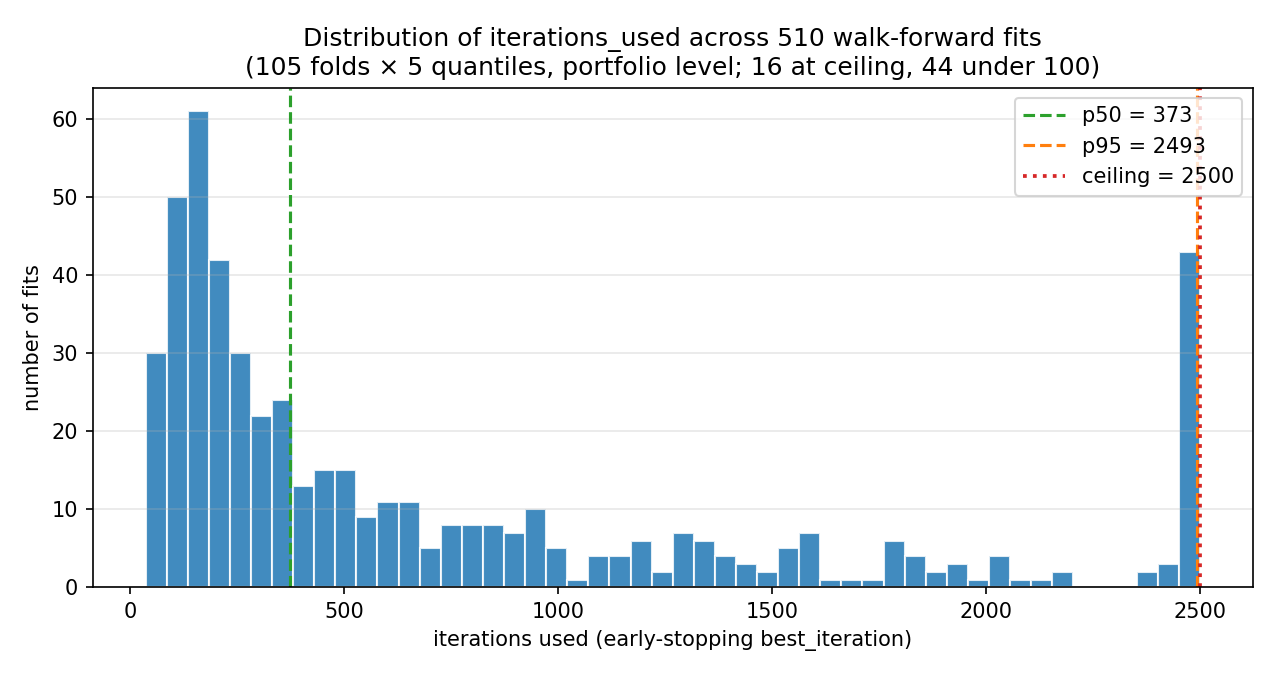
\includegraphics[width=0.92\textwidth]{fig_iters_histogram.png}
\caption{Distribution of \texttt{iterations\_used} (LightGBM
\texttt{best\_iteration}) across 510 walk-forward fits, with the 50th and
95th percentiles and the 2{,}500-round ceiling marked. 16 fits (3.1\%)
hit the ceiling; 44 (8.6\%) stop under 100 iterations.}
\label{fig:iters}
\end{figure}

\subsection{Forecast accuracy by horizon}

Table~\ref{tab:mape} reports walk-forward median MAPE per horizon bucket
and per pointwise horizon for the three competing forecasters: a weekly
persistence baseline ($\hat{y}_t = y_{t-168}$), a SARIMAX baseline with
exogenous block, and the LightGBM portfolio-only suite. The headline
result is MAPE $= 4.88\%$ at $h \leq 24$, ahead of persistence (6.93\%)
and SARIMAX (13.38\%) by margins of 2.05 and 8.50 percentage points
respectively.

\begin{table}[t]
\centering
\caption{Walk-forward median MAPE by horizon, portfolio level, $n =$
total target rows over 102 evaluable folds.}
\label{tab:mape}
\small
\begin{tabular}{l r r r r}
\toprule
horizon & $n$ & persistence & SARIMAX & LightGBM \\
\midrule
$h \leq 24$    & 2{,}448 & 6.93\% & 13.38\% & \textbf{4.88\%} \\
$h = 25\text{--}72$  & 4{,}896 & 6.29\% & 17.44\% & \textbf{5.20\%} \\
$h = 73\text{--}168$ & 9{,}768 & 7.11\% & 23.11\% & \textbf{6.26\%} \\
\midrule
$h = 1$        &   102 & 5.23\% & 16.83\% & \textbf{3.58\%} \\
$h = 24$       &   102 & 4.97\% & 12.09\% & \textbf{4.02\%} \\
$h = 72$       &   102 & \textbf{4.37\%} & 13.69\% & 5.46\% \\
$h = 168$      &   101 & \textbf{5.25\%} & 16.79\% & 6.95\% \\
\bottomrule
\end{tabular}
\end{table}

The LightGBM model wins across all three pool buckets, but the pointwise
breakdown reveals that the win at $h \leq 24$ is decisive (3.58\% at
$h = 1$ vs.\ 5.23\% for persistence) while at $h = 72$ and $h = 168$
LightGBM \emph{loses} to persistence (5.46\% vs.\ 4.37\% and 6.95\% vs.\
5.25\% respectively). We discuss the mechanism in Section~5.4 and as a
limitation in Section~6.

\subsection{Coverage post-conformal}

Table~\ref{tab:coverage} summarizes empirical coverage of the 50\% and
90\% prediction intervals on the test split before and after the
conformal $\delta$ adjustment. The three pool buckets all satisfy the
calibration gate ($[0.45, 0.55]$ for cov\_50, $[0.85, 0.95]$ for
cov\_90) post-calibration. Pre-calibration the recursive bands
substantially undercover at the median horizons: cov\_50 drops to 0.18 at
$h = 25\text{--}72$ and to 0.18 at $h = 73\text{--}168$, with cov\_90
similarly compressed. The conformal adjustments
$\delta(b, q)$ are negative for the lower quantiles and positive for the
upper quantiles, widening the bands by an amount that grows with the
pool's distance from $h = 1$ (median $\delta$ for $q = 0.05$ moves from
$-128$ at $h \leq 24$ to $-216$ at $h = 73\text{--}168$).

\begin{table}[t]
\centering
\caption{Empirical coverage on the test split (51 issue points), raw
recursive bands vs.\ conformal-calibrated bands. The 50\% and 90\%
nominal intervals correspond to $[q_{0.25}, q_{0.75}]$ and
$[q_{0.05}, q_{0.95}]$ respectively.}
\label{tab:coverage}
\small
\begin{tabular}{l r r r r r}
\toprule
bucket & $n$ & raw cov\_50 & cal cov\_50 & raw cov\_90 & cal cov\_90 \\
\midrule
$h \leq 24$    & 1{,}224 & 0.219 & \textbf{0.475} & 0.546 & \textbf{0.899} \\
$h = 25\text{--}72$  & 2{,}448 & 0.184 & \textbf{0.490} & 0.475 & \textbf{0.878} \\
$h = 73\text{--}168$ & 4{,}872 & 0.177 & \textbf{0.482} & 0.463 & \textbf{0.883} \\
\midrule
$h = 1$        &  51 & 0.451 & 0.784 & 0.686 & 0.922 \\
$h = 24$       &  51 & 0.118 & 0.471 & 0.373 & 0.882 \\
$h = 72$       &  51 & 0.020 & 0.471 & 0.314 & 0.824 \\
$h = 168$      &  50 & 0.120 & 0.380 & 0.380 & 0.820 \\
\bottomrule
\end{tabular}
\end{table}

The pointwise diagnostic rows ($h \in \{1, 24, 72, 168\}$) are reported
for transparency but are not part of the calibration gate: the $\delta$
adjustments are computed at the pool-bucket level and within-pool drift
is by design. The visible undercoverage at $h = 168$ (cal cov\_90
$= 0.82$) is the deepest case of within-pool drift and would require
per-horizon adjustments to fix at the cost of much smaller calibration
samples.

Figure~\ref{fig:calibration} plots empirical coverage at the 50\% and
90\% nominal points, raw vs.\ calibrated, for the three pool buckets,
showing the post-calibration trajectories converging close to the
diagonal of perfect calibration.

\begin{figure}[t]
\centering
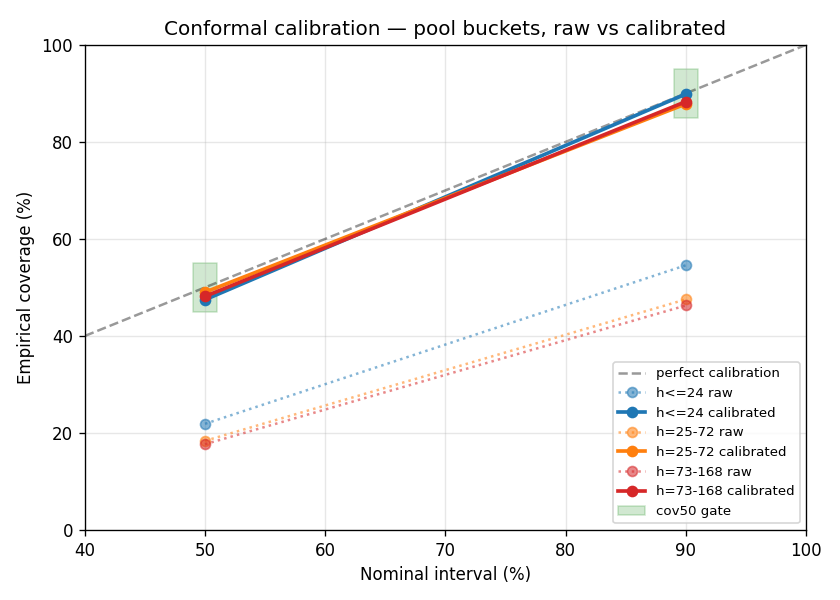
\includegraphics[width=0.85\textwidth]{fig_calibration_curve.png}
\caption{Conformal calibration: empirical coverage versus nominal
interval, raw recursive bands (dotted) and conformal-calibrated bands
(solid), pooled by horizon bucket. Green strips mark the
$[0.45, 0.55] \times [0.85, 0.95]$ acceptance region.}
\label{fig:calibration}
\end{figure}

\subsection{Lift over persistence}

Table~\ref{tab:lift} reports the relative MAPE improvement of LightGBM
over weekly persistence,
$\text{lift} = (\text{MAPE}_{\text{persist}} - \text{MAPE}_{\text{LGB}})\,/\,\text{MAPE}_{\text{persist}}$.

\begin{table}[t]
\centering
\caption{LightGBM relative MAPE improvement over weekly persistence
$\hat{y}_t = y_{t-168}$, by horizon. Negative lift indicates the
LightGBM model loses to the baseline.}
\label{tab:lift}
\small
\begin{tabular}{l r r r}
\toprule
horizon & persistence MAPE & LightGBM MAPE & lift \\
\midrule
$h = 1$        & 5.23\% & 3.58\% & $+31.6\%$ \\
$h \leq 24$    & 6.93\% & 4.88\% & $+29.6\%$ \\
$h = 24$       & 4.97\% & 4.02\% & $+19.1\%$ \\
$h = 25\text{--}72$  & 6.29\% & 5.20\% & $+17.3\%$ \\
$h = 73\text{--}168$ & 7.11\% & 6.26\% & $+12.0\%$ \\
\midrule
$h = 72$       & 4.37\% & 5.46\% & $-25.0\%$ \\
$h = 168$      & 5.25\% & 6.95\% & $-32.4\%$ \\
\bottomrule
\end{tabular}
\end{table}

LightGBM dominates persistence at horizons short enough that the median
recursive prediction has not drifted appreciably from the realized
trajectory. At pointwise $h = 72$ and $h = 168$ the situation reverses:
the recursive median has been folded back as a lag input dozens or
hundreds of times, accumulating per-step error that cannot be undone by
the model's last-step output. Persistence weekly --- which simply copies
the value from one week earlier --- is a remarkably strong baseline at
these horizons because residential consumption is highly periodic at the
weekly scale. This is a structural property of recursive single-step
inference, not a hyperparameter problem; we discuss the implication in
Section~6.

\subsection{Behavioral archetypes}

Figure~\ref{fig:segments} plots the three Pipeline~2 archetypes in the
raw kWh-per-household scale. The \texttt{evening-peak} archetype
(53.4\% of households, 46.4\% of kWh) shows the canonical residential
pattern of low daytime consumption and a 21:00--23:00 peak. The
\texttt{high-baseload} archetype (6.9\% of households, 12.3\% of kWh)
sustains 0.5--0.7~kWh/h through the night and is the highest per-customer
consumer (1.78$\times$ portfolio mean). The \texttt{midday-active}
archetype (39.7\% of households, 41.3\% of kWh) ramps from 09:00 and holds
through the afternoon, consistent with retired households,
work-from-home, and households with day-time caregiving.

\begin{figure}[t]
\centering
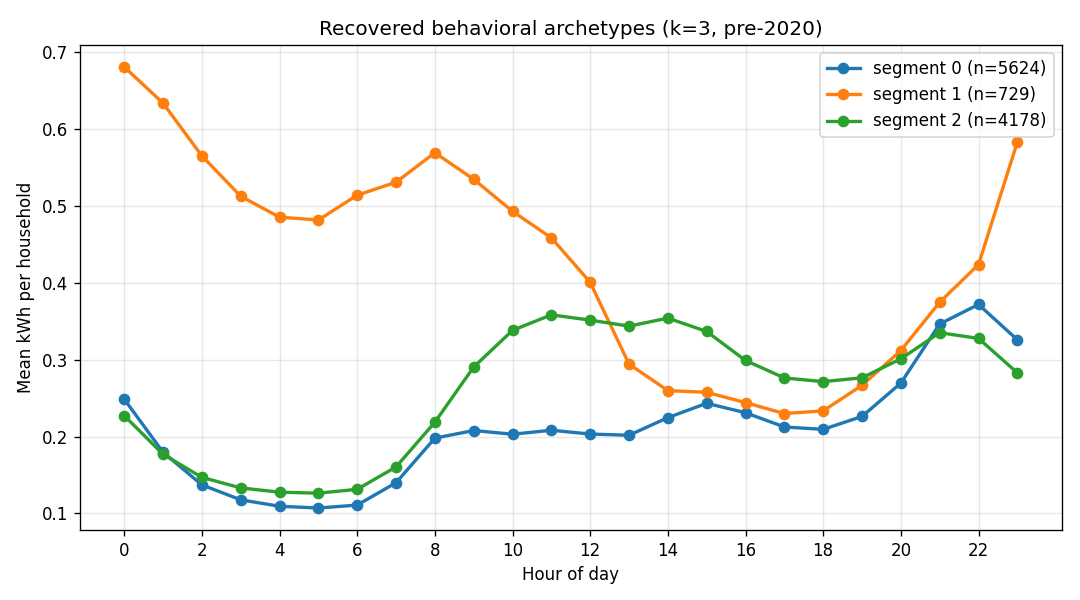
\includegraphics[width=0.85\textwidth]{fig_segment_profiles.png}
\caption{Recovered behavioral archetypes (k-means with $k = 3$,
pre-2020). Each curve plots the within-cluster mean kWh per household by
hour of day in raw kWh; cluster sizes shown in legend.}
\label{fig:segments}
\end{figure}

The commercial reading is straightforward: \texttt{evening-peak} is the
target population for time-of-use tariffs that incentivize off-peak
shifting; \texttt{high-baseload} is the highest-revenue segment per
customer and the natural candidate for retention or premium service
positioning; \texttt{midday-active} is the segment whose load profile
best matches photovoltaic self-consumption and is therefore a natural
target for solar-bundle commercial offers. None of these readings depend
on the silhouette being high; the $k = 3$ partition is operationally
interpretable on the raw kWh scale even when the cluster boundaries are
soft, which they are here.

% =====================================================================
\section{Limitations}
% =====================================================================

\textbf{Recursive error compounding at long horizons.} LightGBM
underperforms persistence at $h = 72$ and $h = 168$ (lift $-25\%$ and
$-32\%$ respectively). The recursive single-step architecture predicts
$\hat{y}_{t+1}$ given features that include past consumption, then folds
$\hat{y}_{t+1}$ back into the lag-1 slot to predict $\hat{y}_{t+2}$, and so
on through the 168-step horizon. The accumulated error is not unbiased
under quantile loss: the per-step residual distribution is fed into a
nonlinear ensemble whose forward error grows superlinearly in step count.
A direct multi-horizon architecture --- one model per horizon, trained on
$y_{t+h} \mid \text{features}(t)$ rather than $y_{t+1}$ --- would address
this at the cost of $7\times$ to $168\times$ more models depending on
horizon granularity. We did not implement it; this is the natural next
iteration.

\textbf{Pinball-loss noise on extreme quantiles.} 8.6\% of fits stop in
fewer than 100 iterations, concentrated at $q = 0.05$ and $q = 0.95$
where the validation pinball loss over a 30-day window is dominated by a
handful of tail observations. Patience $=$ 100 reduces but does not
eliminate this. Two paths forward, both out of scope here: (i)~widen the
validation window to 60 or 90 days, accepting that more recent training
data is sacrificed, or (ii)~replace patience-based early stopping with a
proper Bayesian iteration prior calibrated on prior folds. We document the
rate so it can be revisited if it materially affects deployed coverage.

\textbf{Realized weather in features.} Weather covariates are observed
historical, not forecast. In production, day-ahead and intraday weather
forecasts (with their own error distribution) would replace the realized
series. The MAPE numbers reported here therefore overstate deployed
accuracy by an amount that grows with the contribution of weather features
to the model. Feature-importance aggregation across the five champion
models attributes 20.5\% of total gain to the weather block, so the
expected deployment-time degradation is non-trivial.

\textbf{Iteration ceiling activated.} 3.1\% of fits hit the 2{,}500-round
ceiling, all concentrated at the high-quantile end of the distribution.
This indicates that for some folds the model would have benefited from
more iterations than the cap allowed. Raising the cap to 3{,}500 or
4{,}000 would clear these but at the cost of run time and an unknown
benefit; we kept the cap conservative.

\textbf{Pipeline~2 silhouette below 0.20.} At every $k$ in the sweep, the
silhouette stays below the conventional 0.20 threshold for ``reasonable
structure'' (and well below the 0.50 threshold for ``strong structure'').
Residential daily load shape is a continuum, not a small set of natural
clusters. The $k = 3$ partition is reported as an operational
interpretable carving, not a statistical discovery. Any commercial use of
the labels needs to acknowledge this or risk treating soft, overlapping
groups as if they were strong types.

\textbf{Single-cooperative geographic scope.} The dataset covers one
Spanish cooperative, predominantly Basque Country residential customers.
The portfolio composition (large \texttt{evening-peak} share, small
\texttt{high-baseload} share) is local to that customer base and is not
representative of Spanish residential supply at large, let alone other
markets. External validity claims should be limited accordingly.

% =====================================================================
\section{Operational implications and conclusion}
% =====================================================================

The lift over persistence at $h \leq 24$ (29.6\%) and $h = 25$--$72$
(17.3\%) is large enough to justify adopting LightGBM at the portfolio
level for short-horizon procurement and intraday balancing applications.
The deterioration past $h = 72$ is structural; for week-ahead applications
the weekly persistence baseline $\hat{y}_t = y_{t-168}$ remains
competitive, and we would recommend either using persistence directly at
those horizons or moving to a direct multi-horizon architecture before
deploying recursive single-step at $h = 168$.

Conformal calibration brings the 50\% and 90\% prediction intervals
within 2~percentage points of nominal across the three pool buckets,
satisfying the calibration gate without modifying the median forecast.
Intervals are usable for hedging and reserve sizing under the explicit
caveat that they are calibrated at the pool-bucket level rather than at
each individual horizon, with the largest within-pool drift at $h = 168$
where cov\_90 drops to 0.82.

Pipeline~2 is delivered as a complementary commercial-side artefact: three
operationally interpretable archetypes with explicit silhouette
$< 0.20$ caveat, usable for tariff design and demand-response targeting
but not as feature input to the forecasting pipeline. The two pipelines
share the data ingestion stage but diverge thereafter, which we view as
the correct architectural split given that segmentation for forecasting
and segmentation for commercial use have different success criteria.

The contribution is methodological, not algorithmic: an honest pipeline
documented with its trade-offs, suitable for adoption by other small
operators with similar constraints. Source code, intermediate outputs and
this paper are versioned together in the project repository.

% =====================================================================
\bibliographystyle{plainnat}
\bibliography{refs}
% =====================================================================

\end{document}
